\chapter{Mapa Empático}

    A persona escolhida para criar o mapa empático
    foi a de Fernando, ele tem 37 anos e é o responsável
    pelo armazenamento e monitoramento das vacinas
    nas 5 unidades que a empresa 
    Rio Branco Alimentos SA/Fábrica de Rações de Patrocínio possui.

    Como podemos ver na figura \ref{fig:mapaEmpatico}
    o Fernando esta enfrenando um grave problema na 
    conservação das vacinas de sua empresa.
    No passado já perdeu parte do estoque para esse problema 
    e tem receio que isso volte a acontecer e perder ainda 
    mais produtos, invertimentos e elevar o custo
    e por consequência a credibilidade da 
    empresa perante o mercado.

    Fernando busca uma solução para essa demanda 
    como forma de garantir a qualidade das vacinas e
    manter a credibilidade da empresa e sanar as
    oscilações com relação ao gerenciamento da temperatura
    em todas as unidades.

    \begin{figure}
        \caption{Mapa empático}
        \centering
        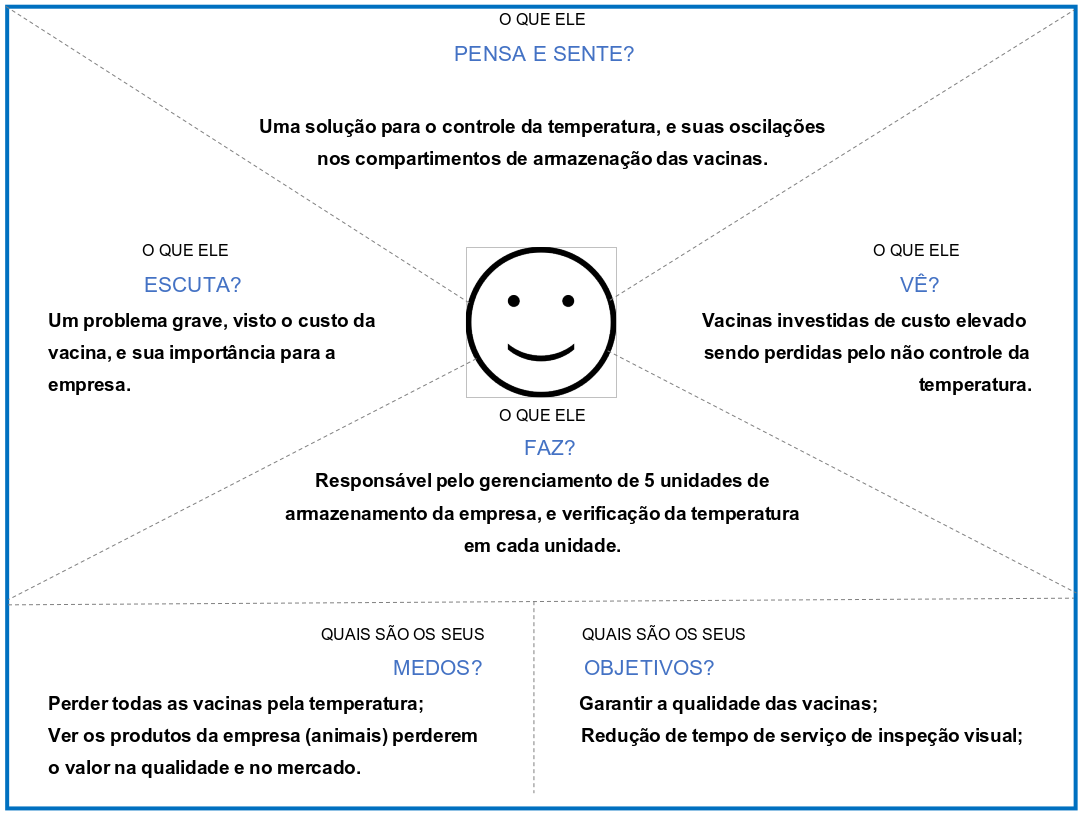
\includegraphics[width=0.85\textwidth]{img/mapa_empatico.png}
        \legend{Fonte: Elaborado pelos autores}
        \label{fig:mapaEmpatico}
    \end{figure}
